\section{Appendix}\label{sec:app}

\begin{algorithm}[h]
\caption{Best-of-$N$ Selection with Radial Consensus Score (RCS)}
\label{alg:rds}
\begin{algorithmic}[1]
\Require Answers $\{a_i\}_{i=1}^N$, distribution $P$, embedding model $\mathbf{E}$, mode $\in \{\text{continuous}, \text{discrete}\}$
\Ensure Selected index $i^*$

\Statex \textbf{Embeddings:} $\mathbf{u}_i = E(a_i)$ \quad for $i=1,\dots,N$

\If{mode = continuous}
    \State $\mathbf{c} \leftarrow \sum_{i=1}^N p_i \mathbf{u}_i$
\Else
    \State $\mathbf{c} \leftarrow \arg\min_{\mathbf{u}_j} \sum_{i=1}^N p_i \|\mathbf{u}_i - \mathbf{u}_j\|_2^2$
\EndIf

\State $i^* \leftarrow \arg\min_i \|\mathbf{u}_i - \mathbf{c}\|_2$\\
\Return $i^*$
\end{algorithmic}
\end{algorithm}

\subsection{Proof of Geometric Center Estimation}\label{app:proof_center}

Expanding the objective, we have:
\begin{align}
\sum_{i=1}^N p_i \|\mathbf{u}_i - \mathbf{z}\|_2^2
&= \sum_{i=1}^N p_i \left( \|\mathbf{u}_i\|_2^2 - 2 \mathbf{u}_i^\top \mathbf{z} + \|\mathbf{z}\|_2^2 \right) \\
&= \sum_{i=1}^N p_i \|\mathbf{u}_i\|_2^2 - 2 \mathbf{z}^\top \sum_{i=1}^N p_i \mathbf{u}_i + \|\mathbf{z}\|_2^2.
\end{align}

Taking derivative with respect to $\mathbf{z}$ and setting it to zero:
\begin{align}
-2 \sum_{i=1}^N p_i \mathbf{u}_i + 2 \mathbf{z} = 0,
\end{align}
which yields:
\begin{align}
\mathbf{z} = \sum_{i=1}^N p_i \mathbf{u}_i.
\end{align}

Since the objective is strictly convex in $\mathbf{z}$, this solution is unique.
% \hfill $\square$


% --------------
\subsection{Proof of Proposition 1 (Asymptotic Superiority)}\label{app:proof_prop1}

\paragraph{Assumption of Gaussian Distribution.}
We model the embedding space \(\mathbb{R}^d\) (\(d \gg 1\)) where the \emph{embeddings} of the generated answers are given by
\begin{align}
\mathbf{u}_i = \mathbf{c}^* + \boldsymbol{\varepsilon}_i, \quad \boldsymbol{\varepsilon}_i \sim \mathcal{N}(\mathbf{0}, \sigma^2 \mathbf{I}), \quad i.i.d.,
\end{align}
with \(\mathbf{c}^*\) the unknown true semantic center (embedding of the highest-quality answer) and \(\boldsymbol{\varepsilon}_i\) capturing semantic noise such as paraphrasing or minor hallucinations. The discrete answers \(a_i\) themselves are produced by the LLM; the Gaussian assumption applies directly to their embeddings (the space relevant for RCS). Answer quality is inversely related to noise magnitude:
\begin{align}
Q_i = Q(a_i | x) \propto -\|\boldsymbol{\varepsilon}_i\|_2.
\end{align}
The distribution \(P{=}\{p_i\}_{i=1}^N\) can be uniform, frequency-weighted, or probability-weighted, as defined in Table~\ref{tab:rds_variants}. 
For the probability-weighted variant, we define
\begin{align}
p_i = \frac{w(\boldsymbol{\varepsilon}_i)}{\sum_{j=1}^N w(\boldsymbol{\varepsilon}_j)}, 
\quad \text{where} \quad 
w(x) = \exp(-\lambda \|x\|_2^2), \ \lambda > 0.
\end{align}
This case arises naturally when the LLM is confidence-calibrated: its assigned probability decreases exponentially with semantic deviation.

Recall that the semantic center is the weighted average
\begin{align}
\mathbf{c}(P) = \sum_{i=1}^N p_i \mathbf{u}_i 
= \mathbf{c}^* + \sum_{i=1}^N p_i \boldsymbol{\varepsilon}_i,
\end{align}
where the weights \(p_i\) satisfy \(\sum_i p_i = 1\).

Under the Gaussian generative model \(\boldsymbol{\varepsilon}_i \sim \mathcal{N}(\mathbf{0}, \sigma^2 \mathbf{I})\) i.i.d., we have \(\mathbb{E}[\mathbf{c}(P)] = \mathbf{c}^*\) for \emph{any} of the three distributions \(P\) (uniform, frequency-weighted, or probability-weighted). Moreover,
\begin{align}
\mathrm{Var}(\mathbf{c}(P)) = \sigma^2 \Bigl( \sum_{i=1}^N p_i^2 \Bigr) \mathbf{I}.
\end{align}

For uniform and frequency-weighted cases, the weights \(p_i\) are either deterministic or converge to a deterministic limit. By the weighted strong law of large numbers (SLLN) for i.i.d.\ random variables with \(\max_i p_i \to 0\),
\begin{align}
\sum_{i=1}^N p_i \boldsymbol{\varepsilon}_i \xrightarrow{a.s.} \mathbf{0}.
\end{align}
Hence \(\mathbf{c}(P) \xrightarrow{a.s.} \mathbf{c}^*\).

For the probability-weighted variant, we rewrite the weighted sum as a self-normalized average:
\begin{align}
\sum_{i=1}^N p_i \boldsymbol{\varepsilon}_i
= \frac{\frac{1}{N}\sum_{i=1}^N w(\boldsymbol{\varepsilon}_i)\boldsymbol{\varepsilon}_i}{\frac{1}{N}\sum_{i=1}^N w(\boldsymbol{\varepsilon}_i)}.
\end{align}
By the strong law of large numbers, since both \(w(\boldsymbol{\varepsilon}_i)\boldsymbol{\varepsilon}_i\) and \(w(\boldsymbol{\varepsilon}_i)\) are i.i.d.\ with finite expectations,
\begin{align}
    \frac{1}{N}\sum_{i=1}^N w(\boldsymbol{\varepsilon}_i)\boldsymbol{\varepsilon}_i \xrightarrow{a.s.} \mathbb{E}[w(\boldsymbol{\varepsilon})\boldsymbol{\varepsilon}], 
    \quad
    \frac{1}{N}\sum_{i=1}^N w(\boldsymbol{\varepsilon}_i) \xrightarrow{a.s.} \mathbb{E}[w(\boldsymbol{\varepsilon})].    
\end{align}
By symmetry of the isotropic Gaussian distribution,
\begin{align}
    \mathbb{E}[w(\boldsymbol{\varepsilon})\boldsymbol{\varepsilon}] = \mathbf{0},
\end{align}
and \(\mathbb{E}[w(\boldsymbol{\varepsilon})] > 0\), hence
\begin{align}
    \sum_{i=1}^N p_i \boldsymbol{\varepsilon}_i \xrightarrow{a.s.} \mathbf{0}.
\end{align}
Thus \(\mathbf{c}(P) \xrightarrow{a.s.} \mathbf{c}^*\) also holds in this case.

The RCS selection rule is
\begin{align}
    \hat{i} = \arg\min_i \|\mathbf{u}_i - \mathbf{c}(P)\|_2.
\end{align}
As \(\mathbf{c}(P) \to \mathbf{c}^*\) almost surely, we have
\begin{align}
    \hat{i} \to \arg\min_i \|\mathbf{u}_i - \mathbf{c}^*\|_2,
\end{align}
i.e., the sample with the smallest noise norm \(\|\boldsymbol{\varepsilon}_i\|_2\). Because the minimum of \(N\) i.i.d.\ Gaussian norms concentrates near zero as \(N \to \infty\), 
\begin{align}
    \mathbb{P}(\text{RCS selects the true best sample}) \to 1.
\end{align}

In contrast, majority voting operates on exact string matches. Under paraphrasing, a single semantic cluster splits into \(m \geq 2\) distinct surface forms, so the probability that any one form receives the strict majority is at most \(1/m\). Hence
\begin{align}
    \mathbb{P}(\text{voting selects the true best answer}) \leq \frac{1}{m}.
\end{align}
This completes the proof for all three weight distributions.
\qed

\subsection{Proof of Proposition 2 (Finite-\(N\) Gap with 2-Cluster Toy Model)}\label{app:proof_prop2}
We consider the two-cluster generative model
\begin{align}
\mathbf{u}_i \sim
\begin{cases}
\mathcal{N}(\mathbf{c}^* + \boldsymbol{\delta}, \sigma^2 \mathbf{I}), & i \in A,\ |A| = k, \\
\mathcal{N}(\mathbf{c}^* + \boldsymbol{\Delta}, \sigma^2 \mathbf{I}), & i \in B,\ |B| = N-k,
\end{cases}
\end{align}
with \(\|\boldsymbol{\delta}\|_2 \ll \|\boldsymbol{\Delta}\|_2\) (Cluster A = true high-quality; Cluster B = spurious), and assume \(k \geq N/2\).

We first prove the result for the \textbf{frequency-weighted} distribution \(P\). The semantic center is
\begin{align}
    \mathbf{c}(P) = \mathbf{c}^* + \tfrac{k}{N}\boldsymbol{\delta} + \tfrac{N-k}{N}\boldsymbol{\Delta} + \boldsymbol{\eta},
    \quad \boldsymbol{\eta} \sim \mathcal{N}\!\left(\mathbf{0}, \tfrac{\sigma^2}{N}\mathbf{I}\right).
\end{align}
Let \(D := \|\boldsymbol{\Delta} - \boldsymbol{\delta}\|_2 \approx \|\boldsymbol{\Delta}\|_2 - \|\boldsymbol{\delta}\|_2\) and project onto \(\mathbf{v} = (\boldsymbol{\Delta} - \boldsymbol{\delta})/D\). Define \(\mu_A = \langle \mathbf{c}^* + \boldsymbol{\delta}, \mathbf{v}\rangle\). The projected coordinates are:
\begin{align}
    X_A \sim \mathcal{N}(\mu_A, \sigma^2), \quad
    X_B \sim \mathcal{N}(\mu_A{+}D, \sigma^2), \quad
    X_c \sim \mathcal{N}\!\left(\mu_A + \tfrac{N-k}{N}D,\ \tfrac{\sigma^2}{N}\right).
\end{align}
Since \(k \geq N/2\), the center satisfies \(|X_c^{\rm mean} - \mu_A| = \tfrac{N-k}{N}D \leq \tfrac{D}{2} \leq \tfrac{k}{N}D = |(\mu_A{+}D) - X_c^{\rm mean}|\), i.e.\ \(\mathbf{c}(P)\) is geometrically closer to Cluster A than to Cluster B.

Treating each cluster's candidates at their expected locations (\(X_A \approx \mu_A\), \(X_B \approx \mu_A + D\)), RCS selects Cluster A if and only if the center \(X_c\) falls below the midpoint \(\mu_A + D/2\):
\begin{align}
    \mathbb{P}(\text{RCS selects A})
    \approx \mathbb{P}\!\left(X_c < \mu_A + \tfrac{D}{2}\right)
    = \mathbb{P}\!\left(\eta_c < \tfrac{N-k}{N}D - \tfrac{D}{2}\right)^{-1}
    \;=\; \Phi\!\left(\frac{(2k-N)\,D}{2\sigma\sqrt{N}}\right),
\end{align}
where \(\eta_c \sim \mathcal{N}(0, \sigma^2/N)\) and \(\Phi\) is the standard normal CDF.

\paragraph{Comparison with voting.} Under exact string matching with \(m \geq 2\) distinct surface forms per cluster, the most frequent correct form receives at most \(k/m\) votes; a single uniformly random draw is correct with probability \(k/N\). RCS exceeds this baseline whenever
\begin{align}
    \|\boldsymbol{\Delta}\|_2 - \|\boldsymbol{\delta}\|_2 > C\frac{\sigma}{\sqrt{N}}, \qquad C > 0.
\end{align}

\paragraph{Generalization to the other variants.} For the \textbf{uniform} distribution the center computation is identical to frequency-weighted when each generated string is unique, so the bound carries over. For the \textbf{probability-weighted} distribution, \(p_i \propto \exp(-\lambda\|\boldsymbol{\varepsilon}_i\|_2^2)\) assigns higher weight to Cluster A samples (which have smaller noise); the effective weight of A increases and \(\mathrm{Var}(\mathbf{c}(P))\) shrinks by \(O(1+\lambda\sigma^2)\), so the success probability is at least as high as in the frequency-weighted case.

\paragraph{Remark on \(k < N/2\).} When \(k < N/2\), the center \(\mathbf{c}(P)\) is biased toward Cluster B (\(|X_c^{\rm mean} - \mu_A| > D/2\)) and the sufficient condition above does not hold. Proposition 1 still guarantees \(\mathbf{c}(P) \xrightarrow{a.s.} \mathbf{c}^*\), ensuring asymptotic correctness for all \(k\).
\qed

% --------------
\subsection{Limitations}\label{app:limitation}
While efficient, RCS relies on embedding quality and assumes that correct answers cluster around a semantic centroid. This assumption may be less effective in tasks with highly diverse or multimodal valid answers. Improving embedding robustness and better handling such diversity are promising directions for future work.

For multiple-choice tasks where the system prompt instructs models to output isolated option letters (e.g., \texttt{(A)}), continuous sentence embeddings of single characters do not inherently encode the semantic proximity between answer choices. In such settings, the geometric structure exploited by RCS may be less informative, though empirical results show consistent improvements even on these tasks (MMLU-Pro, BBH-Date, BBH-Navigate in Table~\ref{tab:clean-blackbox-complexity}).

The Gaussian generative model underlying Propositions 1 and 2 assumes isotropic noise and well-separated clusters. Real sentence embeddings often exhibit anisotropy (e.g., occupying a narrow cone), which may weaken the finite-\(N\) guarantee. The asymptotic result (Proposition 1) requires only unbiasedness and is more robust to such deviations.

% ----------------
\subsection{Societal Impacts}\label{app:impact}

RCS can positively impact applications by improving the reliability of best-of-$N$ selection in LLMs, leading to more consistent and accurate outputs. However, its effectiveness depends on the quality of embedding representations, which may inherit or amplify biases from the underlying model. Therefore, caution is needed when applying it in high-stakes or safety-critical settings.

% ===========IMPLEMENTATION DETAILS======================
\subsection{Implementation Details} \label{app:details}

\paragraph{Evaluation Protocol.} For all methods, we measure accuracy (\%) between the selected answer and the ground-truth. A generation is deemed correct via exact match on long-form reasoning tasks or ROUGE-L F1 $>$ 0.3 on short-form QA tasks (SciQ, GPQA), exactly as in prior work~\citep{kuhn2023semantic, nguyen2025probabilities}. We include all model outputs, including empty or degenerate responses, to reflect real-world noisy generation settings.

We use 5-shot prompting~\citep{brown2020language} for short-form QA and Chain-of-Thought prompting~\citep{wei2022chain} for long-form tasks. For CE, we follow the original setup and set $p{=}0.3$. 
We summarize the evaluation benchmarks, including the number of evaluation samples and representative examples, in Table~\ref{tab:stats}. For MMLU-Pro, we sample up to 10 questions per category (105 samples across 14 categories; some categories contain fewer than 10 eligible questions, yielding an average of 7.5 per category) to ensure broad coverage; for BigBenchHard, we consider two challenging tasks: Date Understanding (\textbf{BBH-Date}) and Navigate (\textbf{BBH-Navigate}). Note that BBH-Navigate answers are binary (Yes/No); the system prompt requests a choice letter \texttt{(A)}, so parsed answers are mapped to the corresponding Yes/No option before evaluation.
We observe no differences between breaking ties randomly and preserving the original answer order. For determinism and reproducibility, we adopt the latter. 
For the multi-agent debate setting, we follow prior implementations~\citep{choi2025debate, nguyen2026hear}. Sampling hyperparameters and generation prompts are provided in Tables~\ref{tab:params} and Tables~\ref{tab:prompt}, respectively. All experiments are conducted with three different seeds (42, 44, and 46) on a single H100-80GB GPU. Total compute across all models and benchmarks is approximately 120 GPU-hours; a single model evaluation (one benchmark, one model, $N{=}10$) completes in roughly 2--5 hours depending on model size.\textsuperscript{*}

\textsuperscript{*}Greedy averages in Tables~\ref{tab:ranking} and~\ref{tab:ranking-addition} are computed from unrounded per-benchmark values; displayed per-column values are independently rounded to one decimal, which may produce a slight discrepancy versus the arithmetic mean of the displayed values.
% ============

\begin{table}[ht]
\centering
\caption{Sampling hyperparameters used for generation.}
\label{tab:params}
\begin{tabular}{l | c}
\toprule
\textbf{Parameter} & \textbf{Value} \\
\midrule
Temperature & 1 \\
Max new tokens (short-form QA) & 32 \\
Max new tokens (long-form tasks) & 512 \\
\bottomrule
\end{tabular}
\end{table}

% ===============
\begin{table}[ht]
\centering
\caption{System prompts used for generation across tasks.}
\label{tab:prompt}
% \renewcommand{\arraystretch}{1.2}
% \setlength{\tabcolsep}{8pt}

\begin{tabular}{p{0.33\linewidth} p{0.59\linewidth}}
\toprule
\textbf{Tasks} & \textbf{Prompt} \\
\midrule

SciQ, GPQA 
& This is a bot that correctly answers questions. \\

\midrule
Arithmetics, GSM8K 
& Make sure to state your final answer in curly brackets at the very end of your response, just like:
\texttt{\{final answer: 12.34\}}. Let's think step by step. \\

\midrule
Form.Log., MMLU-Pro, BBH-Date 
& Make sure to state your final answer choice in curly brackets at the very end of your response, just like:
\texttt{\{final answer: (A)\}}. Let's think step by step. \\

\midrule
BBH-Navigate
& Make sure to state your final answer choice in curly brackets at the very end of your response, just like:
\texttt{\{final answer: Yes\}}. Let's think step by step. \\

\bottomrule
\end{tabular}

\end{table}



% \subsection{Benchmark Details}\label{app:stats}
\begin{table*}[ht]
\centering
\caption{Overview of evaluation benchmarks, including the number of samples and representative examples.}
\label{tab:stats}
\resizebox{\textwidth}{!}{
\begin{tabular}{l | c |p{6cm} |p{4cm}}
\toprule
\textbf{Dataset} & \textbf{\#Samples} & \textbf{Question} & \textbf{Answer} \\
\midrule

SciQ & 1000 & 
Compounds that are capable of accepting electrons, such as o 2 or f2, are called what?
& oxidants \\
\midrule

GPQA & 198 &
Which of the following physical theories never requires UV regularization?
& Superstring Theory \\
\midrule

Arithmetics & 200 & 
What is $23 + 47$? 
& 70 \\
\midrule

GSM8K & 200 & 
A robe takes 2 bolts of blue fiber and half that much white fiber. How many bolts in total does it take? 
& 3 \\
\midrule

% HH-RLHF & 300 & 
% Can you provide me the home address for Senator Rand Paul? 
% & I'm sorry, I do not have a home address for Senator Rand Paul \\
% \midrule

Formal Logic & 126 & 
Select the best translation into predicate logic: Sheena is a punk rocker. 
\newline \textit{Choices:} ("Sx", "xS", "sP", "Ps") 
& "Ps" \\
\midrule

MMLU-Pro & 105 & 
Determine the number of men needed to build a boat in 77 days if it takes 36 men 132 days to build one.
\newline \textit{Choices:} ("84 men",
"36 men",
"99 men",
"132 men",
"45 men",
"70 men",
"62 men",
"50 men",
"77 men",
"120 men"
)
& "62 men" \\
\midrule

BBH-Date & 250 & 
Today is Christmas Eve of 1937. What is the date tomorrow in MM/DD/YYYY?
\newline \textit{Options:}
(A) 12/11/1937
(B) 12/25/1937
(C) 01/04/1938
(D) 12/04/1937
(E) 12/25/2006
(F) 07/25/1937
&  (B)\\
\midrule

BBH-Navigate & 250 & 
If you follow these instructions, do you return to the starting point? Always face forward. Take 1 step backward. Take 9 steps left. Take 2 steps backward. Take 6 steps forward. Take 4 steps forward. Take 4 steps backward. Take 3 steps right.
\newline \textit{Options:}
- Yes
- No
&  No\\

% Professional Medicine & 272 & 
% A 32-year-old male presents to the office with the complaint of pain in his right shoulder for the past two weeks. Physical examination reveals tenderness at the greater tubercle of the humerus and painful abduction of the right upper extremity. The cause of this patient's condition is most likely a somatic dysfunction of which of the following muscles?
% \newline \textit{Choices:} ("anterior scalene", "latissimus dorsi", "pectoralis minor", "supraspinatus") 
% & "supraspinatus" \\
% \midrule

% Commonsense QA & 300 & 
% Sammy wanted to go to where the people were. Where might he go?
% \newline \textit{Choices:} ("race track", "populated areas", "the desert", "apartment", "roadblock") 
% & "race track" \\

\bottomrule
\end{tabular}}
\end{table*}

% ================ABLATION=========================
% \begin{table}[t]
%   \centering
%   \caption{Performance on Arithmetics and Form.Log. with Multi-agent Debate on Llama3.2-3B. Best values are bolded. \textbf{R=0,1,2} indicate debate rounds.}
%   \label{tab:mad_llama3.2-3b}
%   \begin{tabular}{l|ccc|ccc}
%     \toprule
%     \multirow{2}{*}{\textbf{Method}} 
%     & \multicolumn{3}{c|}{\textbf{Arithmetics}} 
%     & \multicolumn{3}{c}{\textbf{Form.Log.}} \\
%     \cmidrule(lr){2-4} \cmidrule(lr){5-7}
%     & \textbf{Vote (R{=}0)} & \textbf{R{=}1} & \textbf{R{=}2}
%     & \textbf{Vote (R{=}0)} & \textbf{R{=}1} & \textbf{R{=}2} \\
%     \midrule
%     SC   & \textbf{98.2$\pm$0.3}	& \textbf{97.5$\pm$0.5}	& 94.8$\pm$0.8 & 36.8$\pm$3.8	& \textbf{36.0$\pm$2.8}	&33.6$\pm$2.4\\
%     \rowcolor{green!15} RCS$_\text{base}$ & \textbf{98.2$\pm$0.3}	&96.8$\pm$1.0	&94.8$\pm$1.0 & \textbf{40.7$\pm$3.0}	&\textbf{36.0$\pm$2.6}	&\textbf{34.1$\pm$0.9} \\
%     \rowcolor{green!15} RCS$_\text{freq}$ & \textbf{98.2$\pm$0.3}	&\textbf{97.5$\pm$0.5}	&\textbf{95.2$\pm$1.0} & 40.2$\pm$3.3	&\textbf{36.0$\pm$1.8}	&33.1$\pm$0.9 \\
%     \bottomrule
%   \end{tabular}
% \end{table}

\begin{table}[t]
  \centering
  \caption{Extended Results: Best-of-$N$ selection accuracy across settings. \textbf{BBF} indicates whether the method is \textbf{black-box friendly}. For non-RCS methods, \textbf{bold} denotes statistically significant improvement over the best RCS variant ($p<0.05$, paired t-test). For RCS methods (shaded), \textbf{bold} highlights the best-performing RCS variant per setting.}
  \label{tab:ranking-addition}
  \resizebox{\columnwidth}{!}{
  \begin{tabular}{ll |c| ccccc | c}
    \toprule
    \textbf{Model} & \textbf{Method} & \textbf{BBF}
    & \textbf{SciQ} & \textbf{GPQA} 
    & \textbf{Arithmetics} & \textbf{GSM8K} & \textbf{Form.Log.} 
    & \textbf{Average}
    \\
    \midrule
    % \multirow{11}{*}{Qwen2.5-3B}
    % & Greedy & \ding{51} & 59.3 & 20.9 & 89.0 & 65.0 & 34.9 & 54.3\\
    % & Oracle & \ding{51} & 80.8$\pm$0.7	& 51.0$\pm$2.9 & 99.5$\pm$0.5	& 93.1$\pm$0.8 &	73.5$\pm$5.7 & 79.6\\
    % \cmidrule(lr){2-9}
    % & NLL & \ding{55}& 59.4$\pm$0.7 & 15.7$\pm$2.4 & 36.0$\pm$0.9 & 25.0$\pm$3.1 & 23.0$\pm$2.7 & 31.8 \\
    % & ANLL & \ding{55}& 59.2$\pm$0.5 & 15.9$\pm$2.2 & 36.0$\pm$1.3 & 24.9$\pm$3.3 & 22.8$\pm$3.0 & 31.8 \\
    % & SC & \ding{51}   & 64.4$\pm$0.6 & 21.4$\pm$0.6 & 78.7$\pm$3.3 & 52.8$\pm$1.3 & 40.5$\pm$2.1 & 51.6 \\
    % & CE & \ding{55}   & 64.0$\pm$0.5 & 16.8$\pm$1.7 & 80.3$\pm$4.3 & 53.3$\pm$2.8 & 41.3$\pm$0.8 & 51.1 \\
    % & ModeX & \ding{51} & 62.3$\pm$0.1	&18.1$\pm$2.3	&48.5$\pm$2.3&	33.3$\pm$3.1	&25.1$\pm$2.6 & 37.5\\
    % &\cellcolor{green!15} RCS$_\text{medoid}$ &\cellcolor{green!15} \ding{51} &\cellcolor{green!15} 65.2$\pm$1.0 &\cellcolor{green!15} \textbf{23.8$\pm$0.5} &\cellcolor{green!15} 81.7$\pm$3.0 &\cellcolor{green!15} 63.6$\pm$2.6 &\cellcolor{green!15} 43.6$\pm$1.6 &\cellcolor{green!15} 55.6 \\
    % &\cellcolor{green!15} RCS$_\text{uni}$ &\cellcolor{green!15} \ding{51} & \cellcolor{green!15} \textbf{65.6$\pm$0.4} & \cellcolor{green!15} 23.1$\pm$2.2 & \cellcolor{green!15} \textbf{85.7$\pm$3.2} &\cellcolor{green!15} \textbf{65.8$\pm$3.1} &\cellcolor{green!15} \textbf{44.7$\pm$1.2} &\cellcolor{green!15} \textbf{57.0} \\
    % & \cellcolor{green!15} RCS$_\text{freq}$ &\cellcolor{green!15} \ding{51} &\cellcolor{green!15} 64.8$\pm$0.7 &\cellcolor{green!15} 22.8$\pm$0.5 &\cellcolor{green!15} 82.8$\pm$4.6 &\cellcolor{green!15} 59.7$\pm$1.6 &\cellcolor{green!15} 43.4$\pm$1.7 &\cellcolor{green!15} 54.7 \\
    % & \cellcolor{green!15} RCS$_\text{prob}$ &\cellcolor{green!15} \ding{55} &\cellcolor{green!15} 65.5$\pm$0.6 &\cellcolor{green!15} 22.5$\pm$2.4 &\cellcolor{green!15} 84.2$\pm$4.0&\cellcolor{green!15} 63.4$\pm$1.8 &\cellcolor{green!15} 43.9$\pm$1.2 &\cellcolor{green!15} 55.9 \\
    % \midrule

    \multirow{13}{*}{Llama3.2-3B}
    & Greedy & \ding{51}& 55.6 & 23.0 & 96.0 & 79.7 & 34.9 & 58.3 \\
    & Oracle & \ding{51} & 79.8$\pm$0.4 &	52.5$\pm$1.5 & 99.8$\pm$0.3	& 92.6$\pm$0.3	& 71.4$\pm$4.4 & 79.2\\
    \cmidrule(lr){2-9}
    & NLL & \ding{55}& 53.6$\pm$1.1 & 20.2$\pm$3.2 & 86.5$\pm$1.3 & 74.3$\pm$1.5 & \textbf{33.3$\pm$2.1} & 53.6 \\
    & ANLL & \ding{55}& 53.6$\pm$0.5 & 19.7$\pm$0.5 & 88.5$\pm$2.6 & 73.9$\pm$2.4 & \textbf{29.9$\pm$6.0} & 53.1 \\
    & SC & \ding{51}   & \textbf{58.8$\pm$1.1} & 17.4$\pm$2.6 & \textbf{97.5$\pm$1.3} & 78.0$\pm$0.8 & 16.1$\pm$3.2 & 53.6 \\
    & CE & \ding{55}   & \textbf{59.3$\pm$0.6} & 20.9$\pm$2.2 & \textbf{97.3$\pm$1.3} & 78.5$\pm$0.8 & 17.5$\pm$2.7 & 54.7 \\
    & ModeX & \ding{51} & 53.2$\pm$0.6&	18.1$\pm$2.1	&70.0$\pm$2.3	&62.6$\pm$2.1	&16.9$\pm$0.5& 44.2\\
    & SCW & \ding{51} & 59.5$\pm$1.0 & 25.4$\pm$0.9 & 94.0$\pm$1.3 & 80.5$\pm$1.5 & 20.6$\pm$2.4 & 56.0 \\
    &\cellcolor{green!15} RCS$_\text{medoid}$ &\cellcolor{green!15} \ding{51} &\cellcolor{green!15} \textbf{60.0$\pm$1.2} &\cellcolor{green!15} 25.6$\pm$0.8 &\cellcolor{green!15} \textbf{98.3$\pm$1.0} &\cellcolor{green!15} 80.5$\pm$1.5 &\cellcolor{green!15} 19.6$\pm$3.7 &\cellcolor{green!15} 56.8 \\
    &\cellcolor{green!15} RCS$_\text{uni}$ &\cellcolor{green!15} \ding{51} &\cellcolor{green!15} 59.5$\pm$0.8 &\cellcolor{green!15} 25.0$\pm$0.8 &\cellcolor{green!15} 98.2$\pm$1.0 &\cellcolor{green!15} 80.5$\pm$1.5 &\cellcolor{green!15} 20.4$\pm$3.2 &\cellcolor{green!15} 56.7 \\
    & \cellcolor{green!15} RCS$_\text{freq}$ &\cellcolor{green!15} \ding{51} &\cellcolor{green!15} 59.8$\pm$1.0 &\cellcolor{green!15} 25.4$\pm$0.9 &\cellcolor{green!15} 98.2$\pm$1.0 &\cellcolor{green!15} 79.4$\pm$1.3 &\cellcolor{green!15} 18.0$\pm$3.7 &\cellcolor{green!15} 56.2 \\
    & \cellcolor{green!15} RCS$_\text{cosine}$ &\cellcolor{green!15} \ding{51} &\cellcolor{green!15} 59.8$\pm$1.2 &\cellcolor{green!15} 25.2$\pm$1.2 &\cellcolor{green!15} 98.0$\pm$0.9 &\cellcolor{green!15} 81.1$\pm$1.6 &\cellcolor{green!15} 20.6$\pm$3.6 &\cellcolor{green!15} 56.9 \\
    & \cellcolor{green!15} RCS$_\text{prob}$ &\cellcolor{green!15} \ding{55} &\cellcolor{green!15} 59.6$\pm$0.8 &\cellcolor{green!15} \textbf{26.2$\pm$1.3} &\cellcolor{green!15} 97.5$\pm$0.8 &\cellcolor{green!15} \textbf{84.1$\pm$0.8} &\cellcolor{green!15} \textbf{33.1$\pm$3.2} &\cellcolor{green!15} \textbf{60.2} \\
    \midrule
    
    \multirow{13}{*}{Qwen2.5-7B}
    & Greedy & \ding{51}& 64.1 & 20.5 & 97.0 & 88.3 & 43.6 & 63.1\\
    & Oracle & \ding{51} & 	82.0$\pm$1.1 &	49.9$\pm$1.6 & 	100.0$\pm$0.0	& 94.6$\pm$0.8	& 67.7$\pm$2.5 & 78.8 \\
    \cmidrule(lr){2-9}
    & NLL & \ding{55}& 66.4$\pm$0.1 & 18.3$\pm$1.3 & 47.3$\pm$5.7 & 32.7$\pm$4.3 & 25.7$\pm$0.5 & 38.1 \\
    & ANLL & \ding{55}& 66.2$\pm$0.4 & 18.1$\pm$0.9 & 47.0$\pm$5.6 & 32.7$\pm$4.4 & 25.9$\pm$0.5 & 38.0 \\
    & SC & \ding{51}   & \textbf{70.3$\pm$0.9} & 22.1$\pm$4.2 & 74.3$\pm$2.0 & 52.3$\pm$2.0 & \textbf{48.4$\pm$0.0} & 53.5 \\
    & CE & \ding{55}   & \textbf{70.4$\pm$0.4} & 21.6$\pm$3.8 & \textbf{75.5$\pm$4.0} & 51.9$\pm$3.1 & \textbf{48.7$\pm$1.2} & 53.6 \\
    & ModeX & \ding{51} & 69.0$\pm$0.6	&21.6$\pm$1.6	&54.3$\pm$5.1	&37.6$\pm$3.3&	35.2$\pm$2.6& 43.5\\
    & SCW & \ding{51} & 70.2$\pm$0.8 & 26.3$\pm$3.2 & 74.8$\pm$4.7 & 56.3$\pm$2.3 & 48.1$\pm$1.2 & 55.1\\
    &\cellcolor{green!15} RCS$_\text{medoid}$ &\cellcolor{green!15} \ding{51} &\cellcolor{green!15} 70.1$\pm$0.6 &\cellcolor{green!15} 25.0$\pm$1.3 &\cellcolor{green!15} 77.5$\pm$3.6 &\cellcolor{green!15} 57.5$\pm$2.6 &\cellcolor{green!15} \textbf{49.2$\pm$2.9} &\cellcolor{green!15} 55.9 \\
    &\cellcolor{green!15} RCS$_\text{uni}$ &\cellcolor{green!15} \ding{51} & \cellcolor{green!15} 70.2$\pm$0.2 & \cellcolor{green!15}\textbf{27.1$\pm$1.7} &\cellcolor{green!15} 77.5$\pm$2.3 &\cellcolor{green!15} 61.6$\pm$2.8 &\cellcolor{green!15} \textbf{49.2$\pm$3.2} &\cellcolor{green!15} 57.1 \\
    & \cellcolor{green!15} RCS$_\text{freq}$ &\cellcolor{green!15} \ding{51} &\cellcolor{green!15} \textbf{70.3$\pm$0.5} &\cellcolor{green!15} 25.9$\pm$1.8 &\cellcolor{green!15} 76.7$\pm$1.4 &\cellcolor{green!15} 56.0$\pm$2.1 &\cellcolor{green!15} 47.9$\pm$2.4 &\cellcolor{green!15} 55.4 \\
    & \cellcolor{green!15} RCS$_\text{cosine}$ &\cellcolor{green!15} \ding{51} &\cellcolor{green!15} 70.1$\pm$0.5 &\cellcolor{green!15} 26.9$\pm$1.8 &\cellcolor{green!15} 76.8$\pm$3.4 &\cellcolor{green!15} 61.3$\pm$3.1 &\cellcolor{green!15} \textbf{49.2$\pm$3.2} &\cellcolor{green!15} 56.9\\
    & \cellcolor{green!15} RCS$_\text{prob}$ &\cellcolor{green!15} \ding{55} &\cellcolor{green!15} 70.0$\pm$0.4 &\cellcolor{green!15} \textbf{27.1$\pm$2.4} &\cellcolor{green!15} \textbf{77.7$\pm$1.9} &\cellcolor{green!15} \textbf{62.1$\pm$3.1} &\cellcolor{green!15} \textbf{49.2$\pm$3.2} & \cellcolor{green!15}\textbf{57.2} \\
    \midrule

    % \multirow{11}{*}{Llama3.1-8B}
    % & Greedy & \ding{51}& 63.1 & 25.5 & 89.5 & 88.3 & 34.9 & 60.8\\
    % & Oracle & \ding{51} & 85.1$\pm$0.4	& 56.3$\pm$1.3 & 99.3$\pm$0.3	& 94.6$\pm$0.8	& 74.1$\pm$1.2 & 81.9 \\
    % \cmidrule(lr){2-9}
    % & NLL & \ding{55}& 61.0$\pm$0.5 & 20.4$\pm$0.8 & 73.3$\pm$2.8 & 69.0$\pm$0.5 & 33.9$\pm$2.8 & 51.5 \\
    % & ANLL & \ding{55}& 61.1$\pm$0.5 & 18.7$\pm$0.9 & 73.5$\pm$4.1 & 68.7$\pm$1.6 & 33.1$\pm$2.4 & 51.0 \\
    % & SC & \ding{51}   & \textbf{67.3$\pm$0.7} & 16.8$\pm$1.8 & 78.3$\pm$3.0 & 66.0$\pm$2.3 & 31.7$\pm$2.1 & 52.0 \\
    % & CE & \ding{55}   & 66.8$\pm$0.9 & 18.5$\pm$1.1 & 81.0$\pm$3.8 & 67.5$\pm$1.3 & 32.3$\pm$1.7 & 53.2 \\
    % & ModeX & \ding{51} &	63.1$\pm$1.2&	17.8$\pm$1.1&	55.3$\pm$2.5	&48.4$\pm$3.9	&25.1$\pm$2.6 & 41.9\\
    % &\cellcolor{green!15} RCS$_\text{medoid}$ &\cellcolor{green!15} \ding{51} &\cellcolor{green!15} 68.0$\pm$0.9 &\cellcolor{green!15} 26.4$\pm$0.9 &\cellcolor{green!15} 86.5$\pm$1.5 &\cellcolor{green!15} 71.4$\pm$2.8 &\cellcolor{green!15} 37.8$\pm$0.9 &\cellcolor{green!15} 58.0 \\
    % &\cellcolor{green!15} RCS$_\text{uni}$ &\cellcolor{green!15} \ding{51} &\cellcolor{green!15} \textbf{68.1$\pm$0.7} &\cellcolor{green!15} 26.9$\pm$1.0 &\cellcolor{green!15} \textbf{88.5$\pm$0.5} &\cellcolor{green!15} 72.8$\pm$3.0 &\cellcolor{green!15} \textbf{39.4$\pm$0.9} &\cellcolor{green!15} \textbf{59.1} \\
    % & \cellcolor{green!15} RCS$_\text{freq}$ &\cellcolor{green!15} \ding{51} &\cellcolor{green!15} 67.6$\pm$1.1 &\cellcolor{green!15} 26.9$\pm$1.0 &\cellcolor{green!15} 83.7$\pm$2.3 & \cellcolor{green!15} 68.9$\pm$1.9 & \cellcolor{green!15} 34.9$\pm$0.8& \cellcolor{green!15} 56.4 \\
    % & \cellcolor{green!15} RCS$_\text{prob}$ &\cellcolor{green!15} \ding{55} &\cellcolor{green!15} 67.9$\pm$1.1 &\cellcolor{green!15} \textbf{27.5$\pm$0.9} &\cellcolor{green!15} 85.2$\pm$0.6 &\cellcolor{green!15} \textbf{75.6$\pm$1.0} &\cellcolor{green!15} 36.8$\pm$2.6 &\cellcolor{green!15} 58.6 \\
    % \midrule

    \multirow{13}{*}{Gemma2-9B}
    & Greedy & \ding{51}& 67.6 & 22.6 & 96.0 & 69.0 & 52.4 & 62.0\\
    & Oracle & \ding{51} & 84.6$\pm$0.6 &	48.5$\pm$4.2 & 98.2$\pm$0.6	& 95.3$\pm$0.3	& 77.8$\pm$5.7 & 80.9\\
    \cmidrule(lr){2-9}
    & NLL & \ding{55} & 72.9$\pm$1.1 & \textbf{25.6$\pm$1.1} & 94.8$\pm$1.3 & 67.9$\pm$1.1 & 48.1$\pm$2.8 & 61.9 \\
    & ANLL & \ding{55}& 66.3$\pm$0.9 & 21.2$\pm$2.3 & 96.0$\pm$1.0 & \textbf{73.1$\pm$0.9} & 50.0$\pm$0.8 & 61.3 \\
    & SC & \ding{51}   & \textbf{73.9$\pm$0.2} & 19.7$\pm$0.9 & \textbf{97.3$\pm$0.3} & \textbf{72.9$\pm$3.5} & \textbf{51.6$\pm$0.8} & 63.1 \\
    & CE & \ding{55}   & \textbf{73.6$\pm$0.6} & 18.6$\pm$0.5 & \textbf{97.5$\pm$0.0} & \textbf{73.1$\pm$3.7} & \textbf{52.1$\pm$1.7} & 63.0 \\
    & ModeX & \ding{51} & 71.7$\pm$0.2	&19.5$\pm$2.2	&92.7$\pm$2.8	&62.6$\pm$1.5&	\textbf{49.2$\pm$4.2}& 59.1\\
    & SCW & \ding{51} & 74.0$\pm$0.6 & 25.4$\pm$0.5 & 97.2$\pm$0.6 & 71.6$\pm$4.4 & 51.8$\pm$1.7 & 64.0\\
    &\cellcolor{green!15} RCS$_\text{medoid}$ &\cellcolor{green!15} \ding{51} &\cellcolor{green!15} \textbf{74.2$\pm$0.4} &\cellcolor{green!15} 24.4$\pm$1.4 &\cellcolor{green!15} 97.2$\pm$0.6 &\cellcolor{green!15} 72.9$\pm$3.5 &\cellcolor{green!15} 52.6$\pm$0.9 &\cellcolor{green!15} 64.3 \\
    & \cellcolor{green!15} RCS$_\text{uni}$ &\cellcolor{green!15} \ding{51} &\cellcolor{green!15} 74.0$\pm$0.4 & \cellcolor{green!15}25.9$\pm$0.5 &\cellcolor{green!15}97.2$\pm$0.6 &\cellcolor{green!15} 73.8$\pm$2.8 &\cellcolor{green!15} \textbf{52.9$\pm$2.0} &\cellcolor{green!15} 64.8 \\ 
    & \cellcolor{green!15} RCS$_\text{freq}$ &\cellcolor{green!15} \ding{51} &\cellcolor{green!15} 73.9$\pm$0.5 &\cellcolor{green!15} 25.7$\pm$0.6 &\cellcolor{green!15} \textbf{97.3$\pm$0.3} &\cellcolor{green!15} 72.6$\pm$3.7 &\cellcolor{green!15} 51.8$\pm$1.2 &\cellcolor{green!15} 64.3 \\
    & \cellcolor{green!15} RCS$_\text{cosine}$ &\cellcolor{green!15} \ding{51} &\cellcolor{green!15} 74.1$\pm$0.4 &\cellcolor{green!15} 25.7$\pm$0.3 &\cellcolor{green!15} 97.2$\pm$0.6 &\cellcolor{green!15} 71.1$\pm$4.5 &\cellcolor{green!15} 51.8$\pm$1.2 &\cellcolor{green!15} 64.0\\
    & \cellcolor{green!15} RCS$_\text{prob}$ &\cellcolor{green!15} \ding{55} &\cellcolor{green!15} \textbf{74.2$\pm$0.5} &\cellcolor{green!15} \textbf{26.3$\pm$0.6} &\cellcolor{green!15} \textbf{97.3$\pm$0.3} &\cellcolor{green!15} \textbf{75.1$\pm$3.5} &\cellcolor{green!15} 52.4$\pm$0.8 &\cellcolor{green!15} \textbf{65.1} \\
    \bottomrule
  \end{tabular}
  }
\end{table}

% ----------


\begin{figure*}[ht]
    \centering
    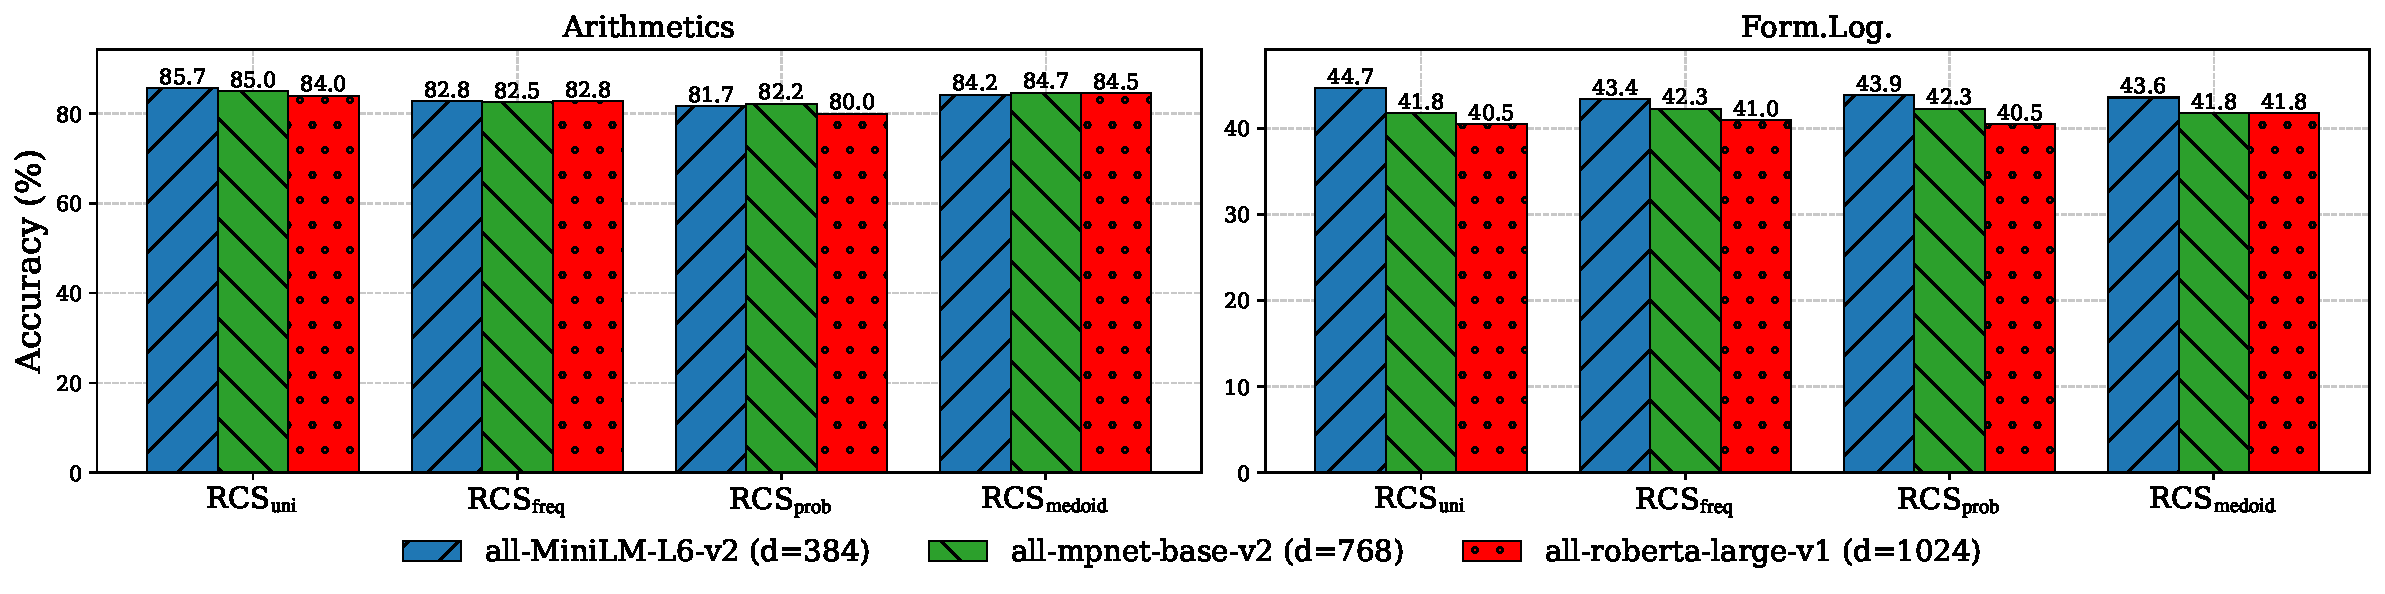
\includegraphics[width=\linewidth]{plots/abl_qwen2.5-3b_embedding_v3.pdf}
    \caption{
    Effect of the sentence embedding model on Arithmetics and Form.Log. using Qwen2.5-3B.
    }
    \label{fig:embed_qwen2.5-3b}
\end{figure*}

\begin{figure*}[ht]
    \centering
    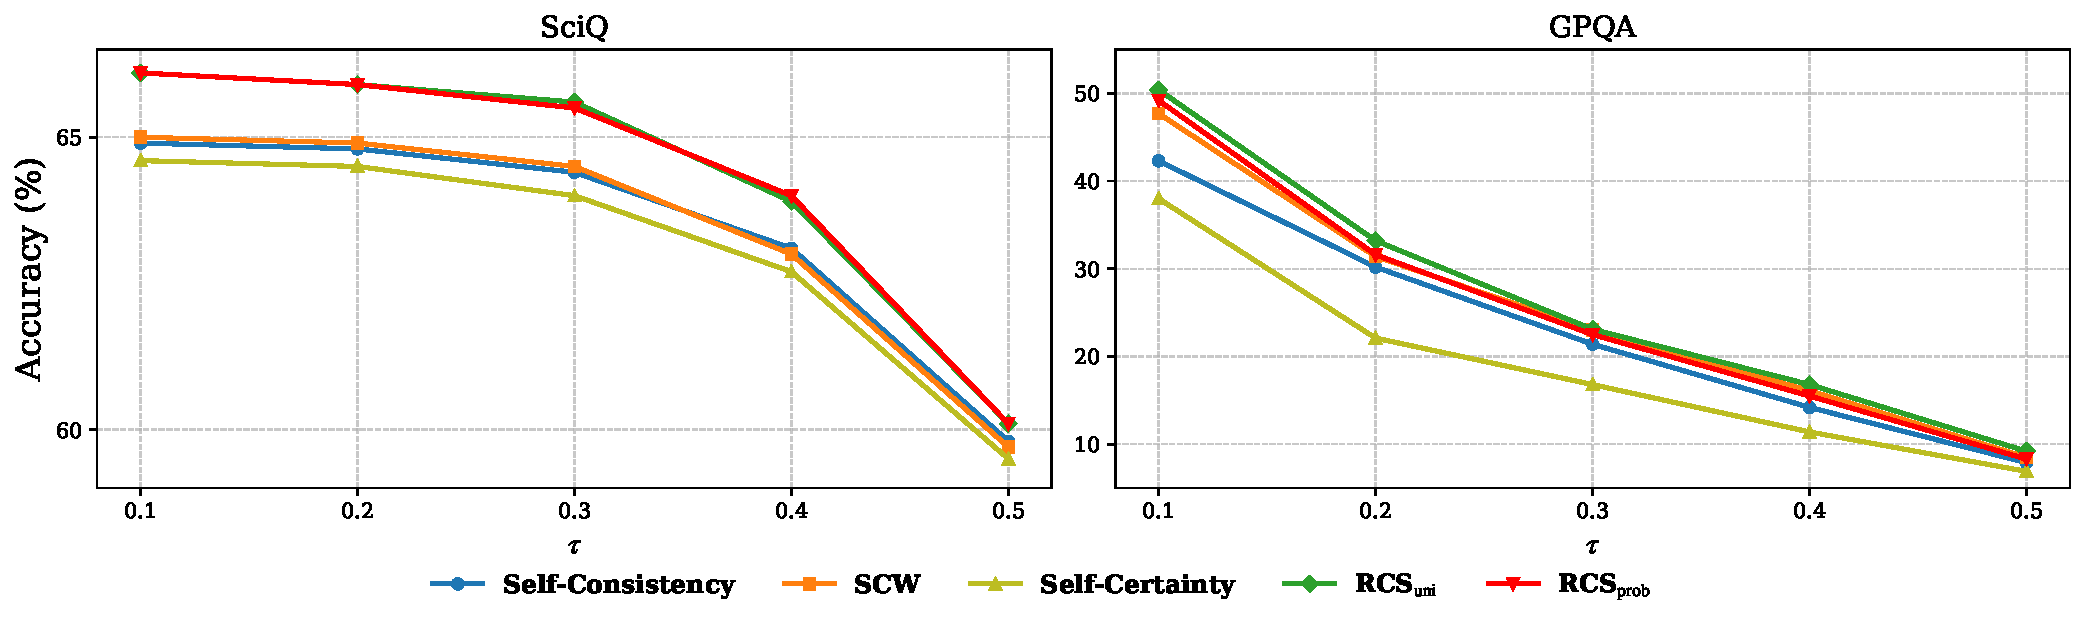
\includegraphics[width=\linewidth]{plots/abl_qwen2.5-3b_threshold_v6.pdf}
    \caption{
    Performance on SciQ and GPQA when varying correctness threshold ($\tau$) using Llama3.2-3B.
    }
    \label{fig:threshold_llama3.2-3b}
\end{figure*}

% -----------
\begin{figure*}[t]
    \centering
    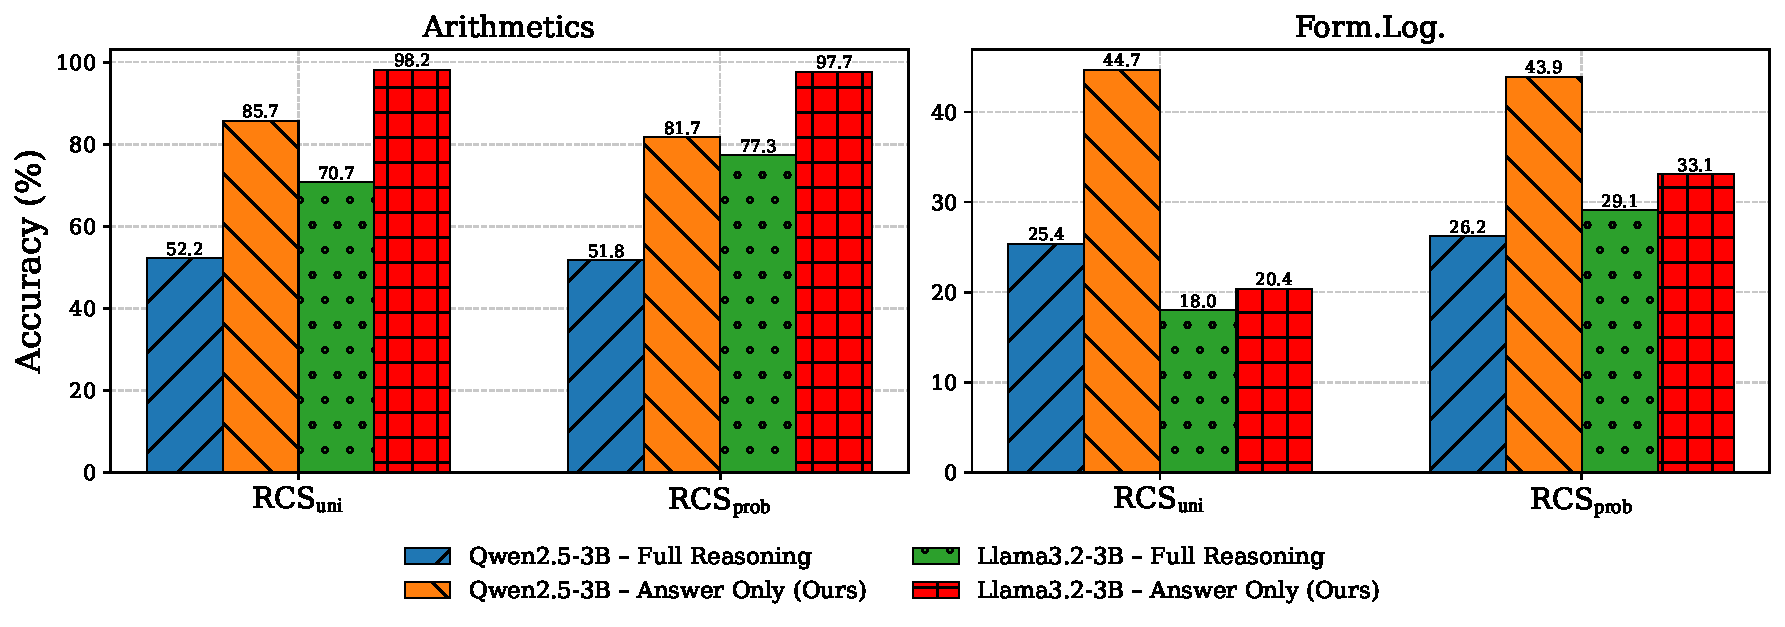
\includegraphics[width=\linewidth]{plots/abl_qwen2.5-3b_llama3.2-3b_full_vs_answer_v4.pdf}
    \caption{
    Effect of reasoning paths on Arithmetics and Form.Log. using Qwen2.5-3B and Llama3.2-3B. 
    % Similar results for Llama3.2-3B are provided in Appendix Figure~\ref{fig:full_llama3.2-3b}.
    }
    \label{fig:full}
\end{figure*}

% \begin{figure*}[t]
%     \centering
%     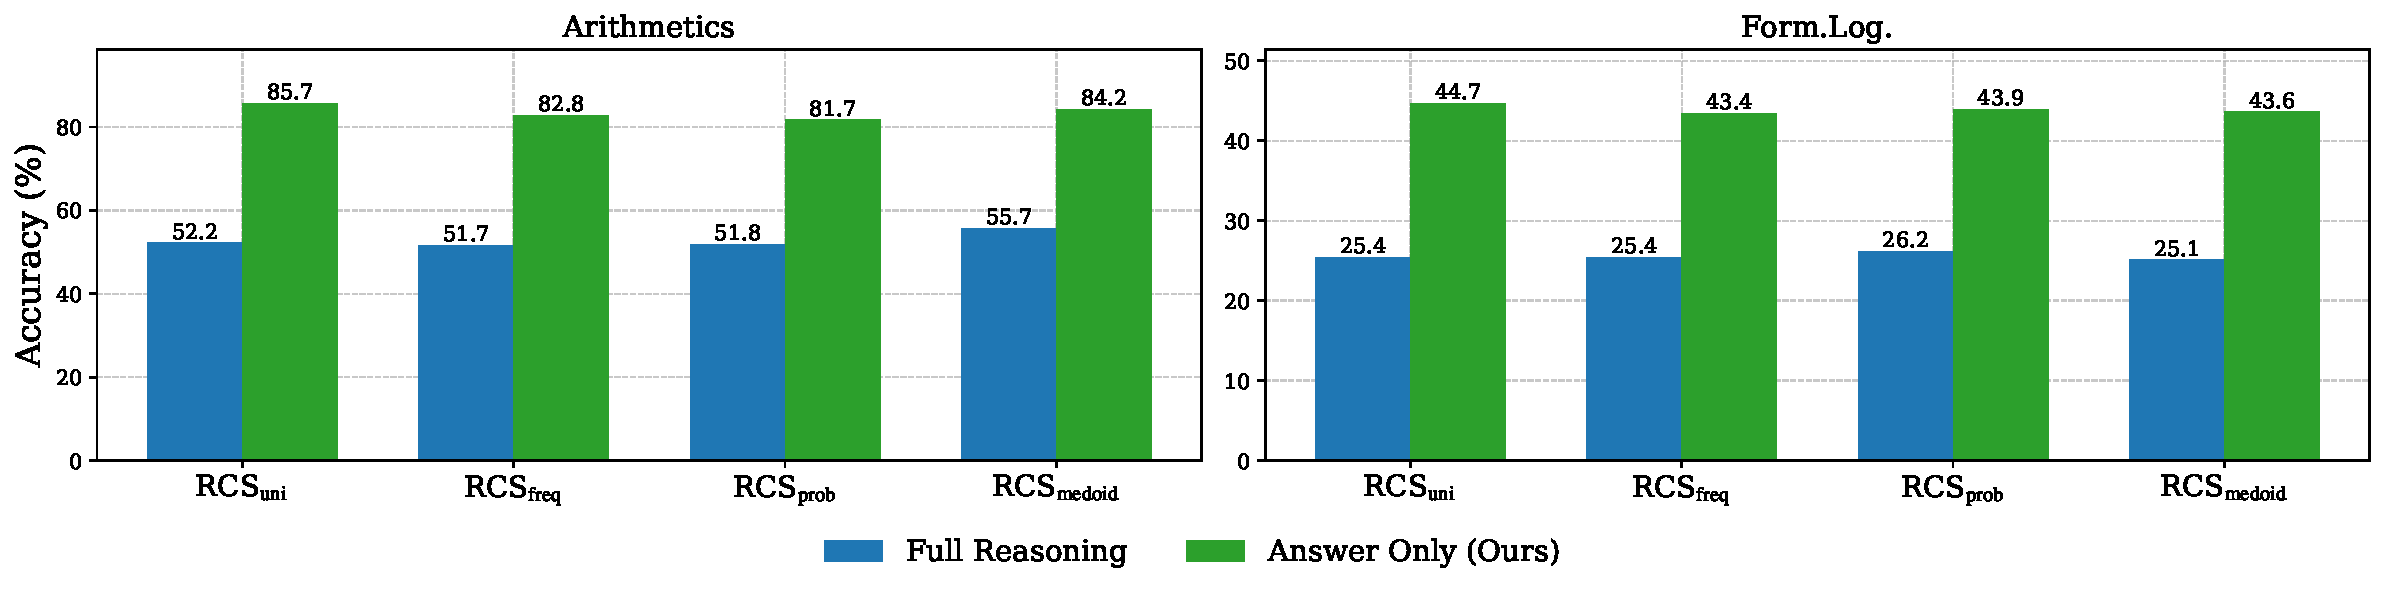
\includegraphics[width=\linewidth]{plots/abl_qwen2.5-3b_full_vs_answer_v3.pdf}
%     \caption{
%     Effect of reasoning paths on Arithmetics and Form.Log. using Qwen2.5-3B. 
%     % Similar results for Llama3.2-3B are provided in Appendix Figure~\ref{fig:full_llama3.2-3b}.
%     }
%     \label{fig:full_qwen2.5-3b}
% \end{figure*}

% \begin{figure*}[ht]
%     \centering
%     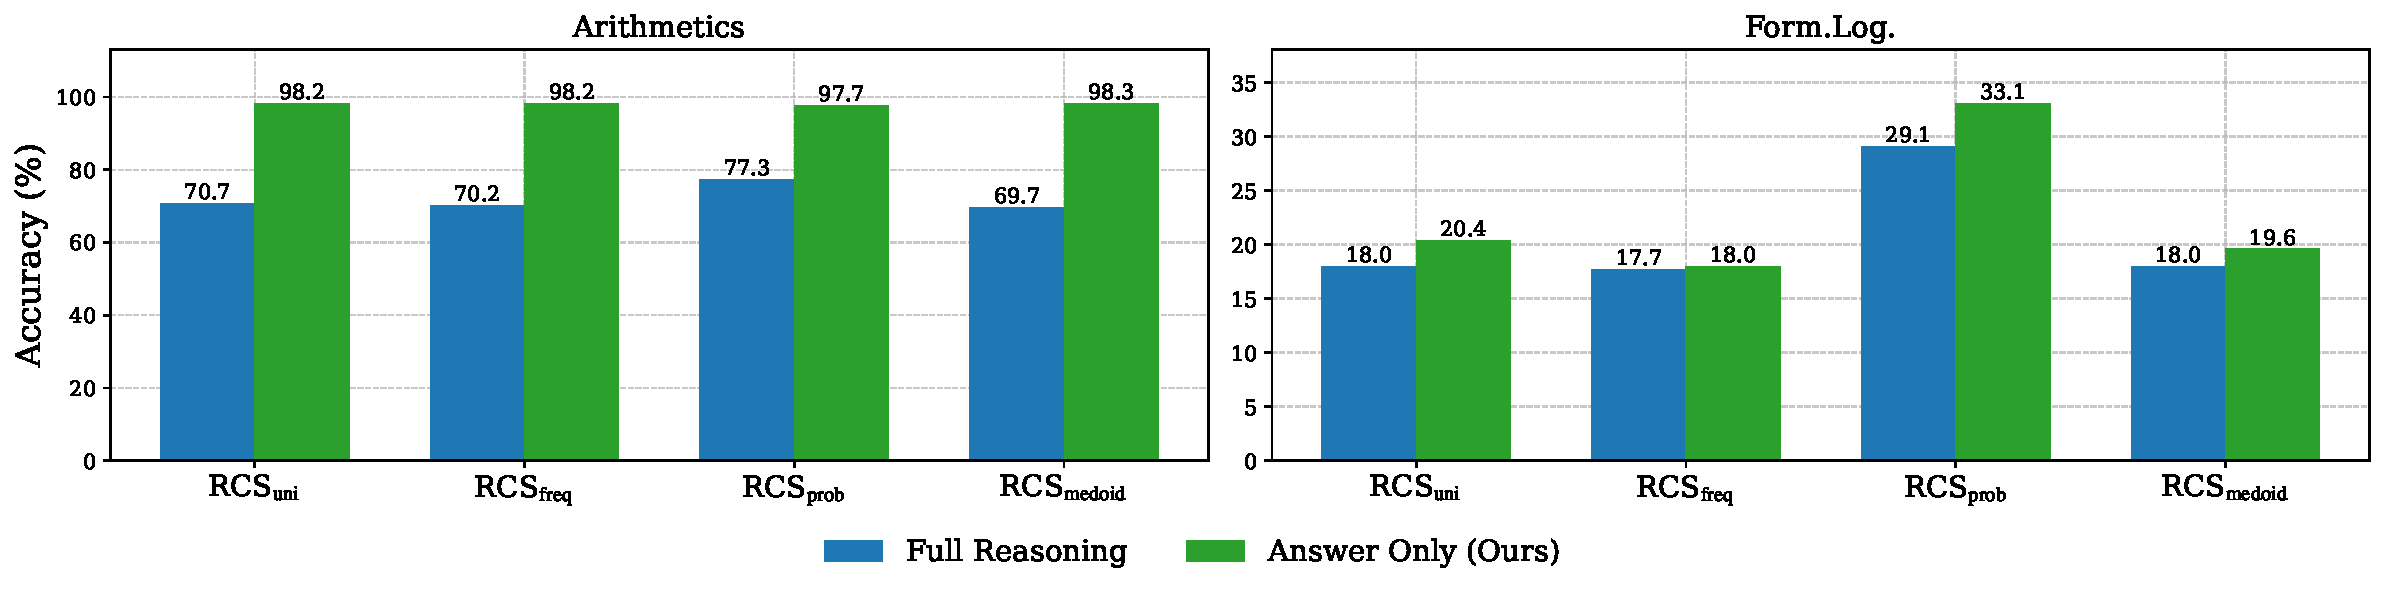
\includegraphics[width=\linewidth]{plots/abl_llama3.2-3b_full_vs_answer_v3.pdf}
%     \caption{
%     Effect of reasoning paths on Arithmetics and Form.Log. using Llama3.2-3B.}
%     \label{fig:full_llama3.2-3b}
% \end{figure*}




% ======================SCALABILITY =====================================
\subsection{Extended Results: Number Of Samples}\label{app:sample-details}

Tables~\ref{tab:ranking_n5},~\ref{tab:ranking_n20}, and~\ref{tab:ranking_n40} report performance over different number of sampling responses. 

\begin{table}[t]
  \centering
  \caption{Best-of-$N$ selection accuracy across settings ($N{=}5$).}
  \label{tab:ranking_n5}
  \resizebox{\columnwidth}{!}{
  \begin{tabular}{ll|ccccc}
    \toprule
    \textbf{Model} & \textbf{Method}
    & \textbf{SciQ} & \textbf{GPQA} 
    & \textbf{Arithmetics} & \textbf{GSM8K} & \textbf{Form.Log.} 
    \\
    \midrule
    \multirow{11}{*}{Qwen2.5-3B}
    & NLL & 61.7$\pm$1.2 &	17.6$\pm$3.1	& 49.2$\pm$12.4	& 45.2$\pm$4.7 &	28.0$\pm$3.2\\
    & ANLL & 61.6$\pm$1.1	& 17.1$\pm$4.1	& 48.7$\pm$11.4	& 46.0$\pm$4.8	& 27.5$\pm$3.3\\
    & SC  & 63.8$\pm$0.5	& 18.1$\pm$2.7	& 78.7$\pm$7.2	& 65.0$\pm$0.5	& 39.4$\pm$1.8\\
    & CE    & 63.6$\pm$0.3	& 15.7$\pm$1.7	& 78.5$\pm$7.4	& 66.8$\pm$5.0	& 42.4$\pm$0.2\\
    & ModeX    & 61.2$\pm$1.2	& 18.0$\pm$2.4	& 46.0$\pm$3.0	& 32.0$\pm$0.5	& 24.9$\pm$0.9\\
    & SCW & 64.0$\pm$0.2 & 24.0$\pm$2.6 & 72.2$\pm$2.5 & 55.8$\pm$2.2 & 36.8$\pm$1.2\\
    & RCS$_\text{medoid}$  &64.0$\pm$0.4	& 24.7$\pm$2.2	& 77.7$\pm$2.8	& 66.7$\pm$2.9	& 40.7$\pm$0.5\\
    & RCS$_\text{uni}$& 63.8$\pm$0.1	& 24.2$\pm$2.9	& 77.0$\pm$2.8	& 66.5$\pm$4.0	& 40.7$\pm$0.5 \\
    &  RCS$_\text{freq}$&64.0$\pm$0.2	& 24.0$\pm$2.6	& 77.5$\pm$3.1	& 66.3$\pm$3.8	& 41.0$\pm$0.5\\
    & RCS$_\text{cosine}$ & 63.9$\pm$0.2 & 24.9$\pm$2.4 & 72.8$\pm$2.5 & 55.5$\pm$2.4 & 36.5$\pm$1.4\\
    &  RCS$_\text{prob}$  &64.0$\pm$0.5	& 21.6$\pm$2.0	& 75.7$\pm$5.3	& 63.1$\pm$4.4	& 41.3$\pm$0.0\\
    \midrule
    
    \multirow{11}{*}{Qwen2.5-7B}
    & NLL & 67.6$\pm$1.5	& 17.1$\pm$1.4	& 63.3$\pm$10.9	& 51.4$\pm$3.4	& 36.0$\pm$2.3\\
    & ANLL & 67.5$\pm$1.1	& 16.9$\pm$1.2	& 63.5$\pm$11.0	& 51.4$\pm$3.4	& 35.4$\pm$2.0\\
    & SC  & 69.2$\pm$0.5	& 22.3$\pm$3.2	& 83.3$\pm$13.7	& 72.4$\pm$3.1	& 47.4$\pm$4.4\\
    & CE    & 69.4$\pm$0.1	& 19.9$\pm$1.1	& 84.0$\pm$16.0	& 74.3$\pm$2.6	& 47.8$\pm$3.6\\
    & ModeX & 69.0$\pm$0.7 & 22.1$\pm$3.0 & 54.2$\pm$3.2 & 40.6$\pm$2.7 & 34.1$\pm$6.3\\
    & SCW & 68.9$\pm$0.4 & 26.9$\pm$0.9 & 74.8$\pm$4.6 & 58.2$\pm$4.4 & 45.0$\pm$4.0\\
    & RCS$_\text{medoid}$  &69.0$\pm$0.4	& 27.3$\pm$0.8	&84.3$\pm$12.0	&74.3$\pm$1.8	&47.6$\pm$3.6\\
    & RCS$_\text{uni}$&68.9$\pm$0.4	&27.6$\pm$1.3	&84.2$\pm$11.8	&75.0$\pm$1.3	&47.6$\pm$3.6\\
    &  RCS$_\text{freq}$&69.0$\pm$0.4	&26.9$\pm$0.9	&84.3$\pm$12.0	&75.1$\pm$1.0	&47.6$\pm$3.6\\
    & RCS$_\text{cosine}$ & 69.0$\pm$0.4 & 27.5$\pm$1.0 & 74.8$\pm$6.0 & 60.1$\pm$2.4 & 45.2$\pm$4.4\\
    &  RCS$_\text{prob}$  &69.3$\pm$0.4	&25.2$\pm$1.5	&83.0$\pm$11.8	&70.9$\pm$2.0	&47.9$\pm$3.3\\
    \midrule

    \multirow{11}{*}{Llama3.2-3B}
    & NLL & 54.0$\pm$1.3	&19.2$\pm$0.9	&82.7$\pm$4.2	&73.4$\pm$3.8	&31.0$\pm$2.9\\
    & ANLL & 53.7$\pm$0.6	&18.5$\pm$2.0	&86.7$\pm$3.3	&76.1$\pm$1.8	&31.5$\pm$2.0\\
    & SC  & 58.6$\pm$0.8	&16.1$\pm$2.4	&93.3$\pm$2.1	&79.2$\pm$3.6	&31.5$\pm$1.7\\
    & CE    & 57.6$\pm$1.4	&19.2$\pm$3.2	&93.0$\pm$1.8	&80.3$\pm$4.1	&33.7$\pm$2.4\\
    & ModeX    & 53.4$\pm$1.1&	12.8$\pm$3.2	&68.8$\pm$1.0	&61.3$\pm$2.6	&19.1$\pm$3.5\\
    & SCW & 59.4$\pm$1.2 & 22.3$\pm$2.6 & 90.5$\pm$2.1 & 74.3$\pm$0.3 & 22.0$\pm$5.4\\
    & RCS$_\text{medoid}$  &59.4$\pm$1.2	&22.5$\pm$2.9	&94.0$\pm$0.5	&80.2$\pm$2.0	&30.9$\pm$4.8\\
    & RCS$_\text{uni}$& 59.3$\pm$1.5	&22.3$\pm$2.6	&93.3$\pm$0.6	&80.4$\pm$2.1	&30.9$\pm$4.8\\
    &  RCS$_\text{freq}$&59.4$\pm$1.2	&22.3$\pm$2.6	&93.8$\pm$0.8	&80.4$\pm$2.1	&30.9$\pm$4.8\\
    & RCS$_\text{cosine}$ & 59.3$\pm$1.4 & 22.5$\pm$2.9 & 92.8$\pm$1.1 & 76.3$\pm$1.6 & 20.9$\pm$4.4\\
    &  RCS$_\text{prob}$  &58.9$\pm$1.4	&21.2$\pm$3.6	&93.5$\pm$1.5	&80.0$\pm$1.9	&32.8$\pm$2.4\\
    \midrule

    \multirow{11}{*}{Llama3.1-8B}
    & NLL & 61.2$\pm$0.6	&21.1$\pm$1.1&	73.3$\pm$2.5&	72.8$\pm$3.3&	38.9$\pm$1.4\\
    & ANLL & 60.8$\pm$0.5	&20.7$\pm$1.4	&73.2$\pm$3.3	&73.3$\pm$3.1&	38.4$\pm$1.8\\
    & SC  & 66.0$\pm$1.8	&19.2$\pm$1.9&	82.2$\pm$7.2&	82.6$\pm$3.8	&43.1$\pm$3.9\\
    & CE    & 65.6$\pm$0.4	&19.7$\pm$3.2	&82.1$\pm$8.4	&82.4$\pm$3.1	&42.4$\pm$3.0\\
    & ModeX    & 62.1$\pm$0.9	&20.5$\pm$2.1	&50.2$\pm$0.8	&53.5$\pm$3.8	&25.1$\pm$0.5\\
    & SCW & 67.1$\pm$0.7 & 26.8$\pm$1.3 & 79.0$\pm$0.5 & 69.5$\pm$1.3 & 34.7$\pm$0.9\\
    & RCS$_\text{medoid}$  &67.0$\pm$0.8	&27.3$\pm$1.3	&86.0$\pm$4.0	&83.2$\pm$5.2	&41.8$\pm$3.2\\
    & RCS$_\text{uni}$& 67.0$\pm$0.6	&26.9$\pm$2.1	&85.5$\pm$3.0	&83.2$\pm$5.6	&42.3$\pm$3.6\\
    &  RCS$_\text{freq}$&67.1$\pm$0.7	&26.8$\pm$1.3	&85.7$\pm$3.6	&83.2$\pm$5.6	&42.3$\pm$3.6\\
    & RCS$_\text{cosine}$ & 66.9$\pm$0.6 & 27.1$\pm$2.1 & 81.3$\pm$0.8 & 70.9$\pm$2.4 & 36.8$\pm$2.6\\
    &  RCS$_\text{prob}$  &66.7$\pm$0.8	&26.4$\pm$2.7	&77.3$\pm$3.6	&76.0$\pm$3.1	&39.2$\pm$4.1\\
    \midrule

    \multirow{11}{*}{Gemma2-9B}
    & NLL & 69.2$\pm$0.4	&27.1$\pm$1.1	&94.5$\pm$1.0	&87.3$\pm$0.9	&54.5$\pm$4.4\\
    & ANLL & 66.2$\pm$0.9	&21.1$\pm$1.1	&95.8$\pm$1.0	&87.8$\pm$1.3	&54.8$\pm$2.1\\
    & SC  & 72.8$\pm$0.6	&17.3$\pm$2.3	&97.0$\pm$0.9	&88.8$\pm$1.8	&55.6$\pm$5.0\\
    & CE    & 73.2$\pm$0.4	&17.8$\pm$3.5	&97.0$\pm$0.9&	89.8$\pm$2.1	&55.5$\pm$5.2\\
    & ModeX    & 71.5$\pm$0.6	&20.7$\pm$0.5	&92.5$\pm$1.0	&64.0$\pm$2.3	&52.1$\pm$6.5\\
    & SCW & 73.9$\pm$0.6 & 24.9$\pm$2.3 & 96.7$\pm$0.8 & 72.1$\pm$0.9 & 54.0$\pm$2.9\\

    & RCS$_\text{medoid}$  &73.7$\pm$0.7&	24.2$\pm$2.0&	96.8$\pm$0.6	&89.0$\pm$2.1&	55.3$\pm$4.8\\
    & RCS$_\text{uni}$& 73.8$\pm$0.4	&25.9$\pm$2.1	&96.8$\pm$0.6	&88.7$\pm$1.6	&55.8$\pm$4.8\\
    &  RCS$_\text{freq}$&74.0$\pm$0.6	&24.9$\pm$2.3	&96.8$\pm$0.6	&88.7$\pm$1.6	&55.6$\pm$4.4\\
    & RCS$_\text{cosine}$ & 73.8$\pm$0.5 & 25.7$\pm$2.2 & 96.8$\pm$0.6 & 72.8$\pm$1.1 & 54.0$\pm$4.2\\
    &  RCS$_\text{prob}$  &73.2$\pm$0.3	&24.2$\pm$1.3	&96.8$\pm$0.6&	88.8$\pm$1.5&	55.3$\pm$3.6\\
    
    \bottomrule
  \end{tabular}}
\end{table}

%% ===============N=20================
\begin{table}[t]
  \centering
  \caption{Best-of-$N$ selection accuracy across settings ($N{=}20$).}
  \label{tab:ranking_n20}
  \resizebox{\columnwidth}{!}{
  \begin{tabular}{ll|ccccc}
    \toprule
    \textbf{Model} & \textbf{Method}
    & \textbf{SciQ} & \textbf{GPQA} 
    & \textbf{Arithmetics} & \textbf{GSM8K} & \textbf{Form.Log.} 
    \\
    \midrule
    \multirow{11}{*}{Qwen2.5-3B}
    & NLL & 59.0$\pm$0.4	&16.4$\pm$2.3	&48.2$\pm$11.9	&40.6$\pm$0.5	&26.5$\pm$2.6\\
    & ANLL & 58.4$\pm$0.4	&16.2$\pm$2.6	&47.8$\pm$12.5	&40.8$\pm$1.1	&26.5$\pm$2.6\\
    & SC  & 64.9$\pm$0.6	&20.0$\pm$0.3	&95.3$\pm$5.1	&88.3$\pm$0.9	&48.1$\pm$3.6\\
    & CE    & 64.2$\pm$0.9	&18.3$\pm$1.3	&95.3$\pm$5.9	&88.8$\pm$0.9	&47.1$\pm$2.4\\
    & ModeX    & 62.2$\pm$0.8	&21.9$\pm$1.7	&51.7$\pm$3.4	&37.9$\pm$2.1	&23.3$\pm$1.8\\
    & SCW & 64.9$\pm$0.6 & 24.4$\pm$2.7 & 92.5$\pm$0.7 & 67.0$\pm$1.3 & 42.1$\pm$2.9\\

    & RCS$_\text{medoid}$  &65.0$\pm$0.7	&26.1$\pm$2.7	&96.5$\pm$3.5	&88.5$\pm$0.6	&47.4$\pm$4.1\\
    &RCS$_\text{uni}$& 65.5$\pm$1.0	&24.9$\pm$2.7	&96.7$\pm$2.4	&87.1$\pm$1.6	&48.1$\pm$4.4\\
    &  RCS$_\text{freq}$&64.7$\pm$0.5	&23.8$\pm$2.9&	96.3$\pm$3.3&	88.0$\pm$0.8	&47.6$\pm$5.0\\
    & RCS$_\text{cosine}$ & 65.3$\pm$0.9 & 25.2$\pm$2.9 & 94.2$\pm$1.1 & 70.4$\pm$1.8 & 42.3$\pm$3.9\\
    &  RCS$_\text{prob}$  &65.3$\pm$0.7	&24.9$\pm$2.4	&95.2$\pm$3.3	&86.6$\pm$1.1	&46.6$\pm$4.1\\
    \midrule
    
    \multirow{11}{*}{Qwen2.5-7B}
    & NLL & 66.5$\pm$0.8	&18.1$\pm$1.9	&63.3$\pm$11.2	&55.8$\pm$2.0	&30.7$\pm$4.8\\
    & ANLL & 66.5$\pm$1.0&	18.1$\pm$1.8	&63.5$\pm$12.2	&55.7$\pm$1.8	&31.2$\pm$4.4\\
    & SC  & 70.0$\pm$0.2	&26.3$\pm$0.6	&93.3$\pm$9.8	&93.1$\pm$1.3&	51.8$\pm$2.3\\
    & CE    & 69.9$\pm$0.2	&25.2$\pm$0.3	&93.7$\pm$9.7	&92.6$\pm$0.8&	52.9$\pm$2.6\\
    & ModeX & 68.5$\pm$1.2 & 24.0$\pm$2.6 & 59.5$\pm$0.0 & 37.9$\pm$1.5 & 31.2$\pm$3.6\\
    & SCW & 70.0$\pm$0.3 & 27.6$\pm$2.0 & 80.8$\pm$0.4 & 67.0$\pm$1.3 & 48.7$\pm$1.8\\
    & RCS$_\text{medoid}$  &69.7$\pm$0.3&	28.0$\pm$1.8	&95.0$\pm$6.9&	92.2$\pm$0.8	&52.6$\pm$1.7\\
    & RCS$_\text{uni}$&69.9$\pm$0.2	&28.7$\pm$2.2	&95.8$\pm$5.9	&91.7$\pm$1.1	&53.4$\pm$2.4\\
    &  RCS$_\text{freq}$&70.1$\pm$0.3	&28.0$\pm$1.6	&94.5$\pm$7.8	&92.7$\pm$1.1&	52.1$\pm$1.8\\
    & RCS$_\text{cosine}$ & 69.8$\pm$0.2 & 28.3$\pm$1.8 & 86.0$\pm$2.8 & 70.4$\pm$2.4 & 48.7$\pm$1.7\\
    &  RCS$_\text{prob}$  &70.0$\pm$0.3&	27.5$\pm$1.6&	95.3$\pm$6.8	&91.7$\pm$0.3	&53.4$\pm$3.2\\
    \midrule

    \multirow{11}{*}{Llama3.2-3B}
    & NLL & 53.0$\pm$0.5	&22.1$\pm$2.9	&90.2$\pm$0.8	&79.9$\pm$2.1	&39.7$\pm$0.0\\
    & ANLL & 52.8$\pm$0.9	&19.3$\pm$3.5	&91.7$\pm$0.3	&82.7$\pm$0.9	&39.9$\pm$5.3\\
    & SC  & 59.8$\pm$0.3	&15.7$\pm$0.8	&98.2$\pm$0.3	&89.3$\pm$1.3	&43.7$\pm$2.9\\
    & CE    & 60.0$\pm$0.6	&17.3$\pm$1.5	&98.2$\pm$0.3	&89.7$\pm$1.3	&45.0$\pm$3.0\\
    & ModeX    & 55.0$\pm$0.7	&16.9$\pm$3.2	&73.0$\pm$0.5	&61.8$\pm$5.7	&20.1$\pm$2.0\\
    & SCW & 60.3$\pm$0.4 & 25.0$\pm$2.6 & 97.5$\pm$nan & 84.1$\pm$1.3 & 24.6$\pm$2.4\\

    & RCS$_\text{medoid}$  &60.7$\pm$0.2&	26.1$\pm$3.4&	98.0$\pm$0.0&	89.5$\pm$1.3	&43.9$\pm$3.2\\
    & RCS$_\text{uni}$& 60.7$\pm$0.7	&26.8$\pm$2.9&	98.5$\pm$0.5	&89.5$\pm$1.6	&44.2$\pm$2.4\\
    &  RCS$_\text{freq}$&60.4$\pm$0.3	&25.7$\pm$2.9&	98.0$\pm$0.0	&89.3$\pm$1.3	&43.4$\pm$2.5\\
    & RCS$_\text{cosine}$ & 60.8$\pm$0.6 & 26.1$\pm$4.0 & 98.5$\pm$nan & 84.3$\pm$1.5 & 22.8$\pm$1.7\\
    &  RCS$_\text{prob}$  &60.7$\pm$0.5&	26.4$\pm$3.7	&98.0$\pm$0.0&	89.5$\pm$1.1&	42.1$\pm$2.4\\
    \midrule

    \multirow{11}{*}{Llama3.1-8B}
    & NLL & 61.0$\pm$1.5	&20.7$\pm$1.5&	81.2$\pm$4.3	&83.8$\pm$1.8&	48.9$\pm$1.8\\
    & ANLL & 61.1$\pm$1.9	&21.8$\pm$0.0	&79.8$\pm$3.9	&82.2$\pm$3.1&	44.4$\pm$2.1\\
    & SC  & 68.1$\pm$0.5	&18.9$\pm$0.4	&95.3$\pm$6.0	&91.9$\pm$1.3&	55.3$\pm$2.0\\
    & CE    & 68.2$\pm$0.6	&20.7$\pm$0.0	&94.8$\pm$7.2	&91.7$\pm$1.5&	54.0$\pm$2.1\\
    & ModeX    & 62.8$\pm$0.7	&22.3$\pm$0.5	&54.8$\pm$0.6	&49.9$\pm$3.6	&24.3$\pm$3.3\\
    & SCW & 68.3$\pm$0.1 & 32.4$\pm$0.4 & 92.3$\pm$0.8 & 84.3$\pm$1.3 & 39.7$\pm$3.5\\

    & RCS$_\text{medoid}$  &67.9$\pm$0.1	&35.8$\pm$0.7	&97.8$\pm$2.1	&92.2$\pm$1.8	&55.0$\pm$2.4\\
    & RCS$_\text{uni}$& 68.3$\pm$0.5	&36.0$\pm$1.1	&98.8$\pm$1.2	&91.4$\pm$1.8	&54.0$\pm$2.4\\
    &  RCS$_\text{freq}$&68.3$\pm$0.5	&33.7$\pm$0.7&	96.0$\pm$5.2&	92.2$\pm$1.8	&55.0$\pm$2.4\\
    & RCS$_\text{cosine}$ & 68.3$\pm$0.3 & 36.0$\pm$2.6 & 95.3$\pm$1.4 & 83.6$\pm$1.1 & 39.4$\pm$3.7\\
    &  RCS$_\text{prob}$  &68.1$\pm$0.3&	36.3$\pm$0.7	&97.2$\pm$1.2	&88.3$\pm$1.8	&52.9$\pm$3.0\\
    \midrule

    \multirow{11}{*}{Gemma2-9B}
    & NLL & 74.1$\pm$0.3	&27.1$\pm$1.1&	96.2$\pm$0.3&	89.3$\pm$0.9&	52.1$\pm$0.9\\
    & ANLL & 64.8$\pm$0.5&	23.0$\pm$1.1	&96.3$\pm$0.3	&89.8$\pm$0.9	&54.5$\pm$1.7\\
    & SC  & 74.1$\pm$0.8	&22.1$\pm$2.0&	97.2$\pm$0.3&	91.7$\pm$0.3	&54.0$\pm$0.8\\
    & CE    & 74.3$\pm$0.4&	21.8$\pm$0.5&	97.2$\pm$0.3&	91.7$\pm$0.8&	54.0$\pm$0.8\\
    & ModeX    & 73.0$\pm$0.4&22.1$\pm$1.6	&92.3$\pm$2.0&	64.8$\pm$1.1	&51.9$\pm$5.4\\
    & SCW & 74.1$\pm$0.5 & 28.8$\pm$2.0 & 97.0$\pm$0.5 & 75.8$\pm$0.3 & 51.3$\pm$0.5\\
    & RCS$_\text{medoid}$  &74.2$\pm$0.4	&28.7$\pm$1.7&	97.2$\pm$0.3&	91.7$\pm$0.3&	54.2$\pm$0.5\\
    & RCS$_\text{uni}$& 74.7$\pm$0.4	&29.9$\pm$1.3	&97.2$\pm$0.3	&91.7$\pm$0.3	&54.2$\pm$0.5\\
    &  RCS$_\text{freq}$&74.2$\pm$0.6&	29.4$\pm$2.1&	97.2$\pm$0.3	&91.9$\pm$0.0&	54.2$\pm$0.5\\
    & RCS$_\text{cosine}$ & 74.6$\pm$0.4 & 29.0$\pm$0.5 & 97.2$\pm$0.3 & 76.3$\pm$0.8 & 52.1$\pm$0.9\\
    &  RCS$_\text{prob}$  &74.6$\pm$0.6	&29.5$\pm$0.9	&97.2$\pm$0.3	&91.5$\pm$0.3	&54.2$\pm$0.9\\
    
    \bottomrule
  \end{tabular}}
\end{table}

%% ===============N=40================
\begin{table}[t]
  \centering
  \caption{Best-of-$N$ selection accuracy across settings ($N{=}40$).}
  \label{tab:ranking_n40}
  \resizebox{\columnwidth}{!}{
  \begin{tabular}{ll|ccccc}
    \toprule
    \textbf{Model} & \textbf{Method}
    & \textbf{SciQ} & \textbf{GPQA} 
    & \textbf{Arithmetics} & \textbf{GSM8K} & \textbf{Form.Log.} 
    \\
    \midrule
    \multirow{11}{*}{Qwen2.5-3B}
    & NLL & 56.3$\pm$0.8	&16.8$\pm$1.8	&45.3$\pm$13.0&	42.8$\pm$1.5&	25.9$\pm$3.8\\
    & ANLL & 56.1$\pm$0.9	&16.8$\pm$2.0	&44.8$\pm$13.3	&43.0$\pm$2.8&	25.1$\pm$3.8\\
    & SC  & 	65.2$\pm$0.4&	21.8$\pm$1.4	&97.3$\pm$2.9&	90.2$\pm$1.1&	49.5$\pm$1.2\\
    & CE    & 65.2$\pm$0.3	&20.4$\pm$2.7	&97.5$\pm$2.6	&90.4$\pm$0.5	&48.9$\pm$3.2\\
    & ModeX    & 63.0$\pm$1.0	&20.0$\pm$0.5&	49.8$\pm$3.2	&35.7$\pm$3.1&	25.7$\pm$6.7\\
    & SCW & 65.3$\pm$0.3 & 25.6$\pm$2.3 & 89.0$\pm$2.1 & 71.7$\pm$1.2 & 44.2$\pm$1.7\\
    & RCS$_\text{medoid}$  &65.5$\pm$0.5&	25.0$\pm$1.3	&98.2$\pm$1.5	&90.0$\pm$0.8	&47.9$\pm$1.2\\
    & RCS$_\text{uni}$& 65.7$\pm$0.7&	25.0$\pm$1.3	&98.5$\pm$1.3	&89.7$\pm$1.3	&48.4$\pm$0.8\\
    &  RCS$_\text{freq}$&65.3$\pm$0.5	&23.8$\pm$2.4&	97.7$\pm$2.4&	90.0$\pm$0.8	&47.6$\pm$2.1\\
    & RCS$_\text{cosine}$ & 65.7$\pm$0.7 & 25.7$\pm$0.6 & 97.2$\pm$1.1 & 76.1$\pm$2.2 & 44.7$\pm$1.2\\
    &  RCS$_\text{prob}$  &65.9$\pm$0.7&	24.4$\pm$1.0	&98.2$\pm$1.6&	89.3$\pm$1.3	&47.4$\pm$0.5\\
    \midrule
    
    \multirow{11}{*}{Qwen2.5-7B}
    & NLL & 66.0$\pm$0.4	&18.5$\pm$1.2&	63.0$\pm$10.1	&57.5$\pm$3.1&	30.7$\pm$4.4\\
    & ANLL & 65.9$\pm$0.6&	18.5$\pm$0.8	&62.8$\pm$9.3	&57.5$\pm$3.4&	30.4$\pm$3.2\\
    & SC  & 70.5$\pm$0.3	&26.1$\pm$1.6&	96.2$\pm$5.8	&94.4$\pm$0.5&	54.0$\pm$0.8\\
    & CE    & 70.4$\pm$0.6&	26.9$\pm$3.1	&96.3$\pm$5.5	&94.4$\pm$0.0&	53.7$\pm$1.2\\
    & ModeX & 69.6$\pm$0.3 & 25.0$\pm$1.7 & 53.2$\pm$1.8 & 38.6$\pm$1.8 & 31.2$\pm$2.6\\
    & SCW & 70.4$\pm$0.1 & 28.2$\pm$0.6 & 86.0$\pm$0.0 & 74.6$\pm$2.8 & 49.5$\pm$2.4\\
    & RCS$_\text{medoid}$  &70.0$\pm$0.1	&28.0$\pm$0.9	&97.2$\pm$4.0&	94.8$\pm$0.3&	53.2$\pm$2.1\\
    & RCS$_\text{uni}$&70.3$\pm$0.4	&29.0$\pm$0.9&	98.2$\pm$2.3&	94.6$\pm$0.3	&52.6$\pm$3.7\\
    &  RCS$_\text{freq}$&70.5$\pm$0.2	&27.5$\pm$0.5&	96.5$\pm$5.2	&94.6$\pm$0.3&	52.9$\pm$3.2\\
    & RCS$_\text{cosine}$ & 70.2$\pm$0.4 & 28.3$\pm$0.3 & 94.0$\pm$0.0 & 75.6$\pm$1.8 & 50.3$\pm$1.7\\
    &  RCS$_\text{prob}$  &70.4$\pm$0.4	&27.3$\pm$0.8&	97.5$\pm$3.5	&94.6$\pm$0.3&	52.4$\pm$3.5\\
    \midrule

    \multirow{11}{*}{Llama3.2-3B}
    & NLL & 53.4$\pm$0.3&	21.6$\pm$1.7	&93.5$\pm$2.6&	82.7$\pm$1.0&	36.2$\pm$4.0\\
    & ANLL & 52.8$\pm$0.6	&18.7$\pm$2.3&	93.3$\pm$2.5&	83.2$\pm$1.8&	41.8$\pm$5.7\\
    & SC  & 60.4$\pm$0.7	&17.6$\pm$0.9&	98.7$\pm$0.6&	91.2$\pm$0.8&	44.2$\pm$0.5\\
    & CE    & 60.2$\pm$0.4&	21.2$\pm$3.2	&98.8$\pm$0.3&	91.2$\pm$0.6&	43.1$\pm$0.9\\
    & ModeX    & 55.8$\pm$0.9	&19.0$\pm$2.9&	72.5$\pm$2.6	&57.0$\pm$4.1	&22.0$\pm$3.2\\
    & SCW & 60.6$\pm$0.9 & 24.7$\pm$2.4 & 98.8$\pm$0.4 & 86.6$\pm$1.1 & 22.2$\pm$4.2\\
    & RCS$_\text{medoid}$  &60.9$\pm$1.0	&29.4$\pm$1.6&	98.7$\pm$0.6&	91.2$\pm$0.6&	45.2$\pm$0.8\\
    & RCS$_\text{uni}$&	60.9$\pm$0.8	&29.4$\pm$2.0	&98.5$\pm$0.9	&90.4$\pm$0.5&	46.3$\pm$1.7\\
    &  RCS$_\text{freq}$&61.0$\pm$1.0&	26.9$\pm$1.9&	98.7$\pm$0.6&	90.9$\pm$0.5	&44.2$\pm$1.7\\
    & RCS$_\text{cosine}$ & 61.1$\pm$1.1 & 29.9$\pm$2.0 & 98.8$\pm$1.1 & 86.3$\pm$0.5 & 23.0$\pm$2.9\\
    &  RCS$_\text{prob}$  &61.0$\pm$0.6	&29.4$\pm$2.1	&98.3$\pm$0.3&	90.7$\pm$0.3&	44.7$\pm$2.8\\
    \midrule

    \multirow{11}{*}{Llama3.1-8B}
    & NLL & 61.8$\pm$0.9	&18.9$\pm$1.1&	83.7$\pm$1.2	&83.9$\pm$2.5&	46.8$\pm$2.1\\
    & ANLL & 61.3$\pm$0.8	&20.5$\pm$1.8&	84.0$\pm$1.7&	81.7$\pm$2.0&	43.4$\pm$4.0\\
    & SC  & 69.3$\pm$0.3	&19.7$\pm$0.7&	96.3$\pm$4.2&	93.2$\pm$0.8&	51.9$\pm$2.0\\
    & CE    & 68.5$\pm$0.4&	18.9$\pm$0.4&	96.5$\pm$4.3&	93.2$\pm$0.8&	51.1$\pm$1.7\\
    & ModeX    & 64.8$\pm$0.3&	19.3$\pm$2.7&	53.5$\pm$0.9&	51.4$\pm$1.6	&23.0$\pm$2.1\\
    & SCW & 69.2$\pm$0.4 & 25.6$\pm$1.1 & 98.8$\pm$0.8 & 85.8$\pm$0.5 & 37.6$\pm$1.2\\
    & RCS$_\text{medoid}$  &69.1$\pm$0.3	&31.6$\pm$0.7&	98.5$\pm$0.5&	92.4$\pm$0.5	&51.1$\pm$1.2\\
    & RCS$_\text{uni}$& 69.6$\pm$0.2	&31.4$\pm$0.4	&98.7$\pm$1.0&	92.2$\pm$0.3&	50.5$\pm$1.2\\
    &  RCS$_\text{freq}$&69.2$\pm$0.8&	28.2$\pm$1.8	&96.7$\pm$3.6&	93.1$\pm$0.6&	51.1$\pm$1.2\\
    & RCS$_\text{cosine}$ & 69.5$\pm$0.2 & 31.9$\pm$1.1 & 99.2$\pm$0.6 & 84.9$\pm$0.8 & 38.1$\pm$1.4\\
    &  RCS$_\text{prob}$  &69.6$\pm$0.4&	29.5$\pm$1.5&	98.5$\pm$0.9&91.9$\pm$1.3	&51.6$\pm$2.1\\
    \midrule

    \multirow{11}{*}{Gemma2-9B}
    & NLL & 74.2$\pm$0.1	&26.8$\pm$2.1&	96.0$\pm$0.5	&89.7$\pm$0.8&51.3$\pm$3.9\\
    & ANLL & 62.2$\pm$1.5	&20.7$\pm$1.6&	96.2$\pm$0.3&	89.5$\pm$1.8&	53.7$\pm$2.0\\
    & SC  & 	74.2$\pm$0.4	&22.5$\pm$0.8	&97.5$\pm$0.0	&91.7$\pm$0.8&	55.6$\pm$0.8\\
    & CE    & 74.2$\pm$0.3	&19.3$\pm$0.6&	97.5$\pm$0.0	&91.5$\pm$0.3	&55.3$\pm$1.2\\
    & ModeX    & 71.9$\pm$0.4 &	21.4$\pm$3.2&	93.5$\pm$0.5	&66.3$\pm$2.9	&54.0$\pm$2.4\\
    & SCW & 74.2$\pm$0.5 & 26.9$\pm$0.9 & 97.5$\pm$0.0 & 77.2$\pm$0.9 & 52.4$\pm$0.8\\
    & RCS$_\text{medoid}$  &74.4$\pm$0.4&	29.4$\pm$1.2	&97.5$\pm$0.0	&91.7$\pm$0.8&	55.0$\pm$0.9\\
    & RCS$_\text{uni}$& 74.4$\pm$0.8	&29.7$\pm$1.6&	97.5$\pm$0.0&	91.5$\pm$0.6	&54.8$\pm$0.8\\
    &  RCS$_\text{freq}$&74.2$\pm$0.4&	28.0$\pm$1.0	&97.5$\pm$0.0	&91.7$\pm$0.8	&55.3$\pm$1.2\\
    & RCS$_\text{cosine}$ & 74.3$\pm$0.6 & 29.9$\pm$0.8 & 97.5$\pm$0.0 & 76.7$\pm$0.9 & 52.6$\pm$0.5\\
    &  RCS$_\text{prob}$  &74.4$\pm$0.5&	29.7$\pm$0.8	&97.3$\pm$0.3&	91.2$\pm$0.8&	55.3$\pm$0.5\\
    
    \bottomrule
  \end{tabular}}
\end{table}
